\documentclass[a4paper, 10pt, final, garamond]{book}
\usepackage{cours-preambule}
\graphicspath{{./figures/}}

\makeatletter
\renewcommand{\@chapapp}{Contr\^ole de connaissances}
\makeatother

% \toggletrue{student}
% \HideSolutionstrue
% \toggletrue{corrige}
\renewcommand{\mycol}{black}

\begin{document}
\setcounter{chapter}{10}

\chapter{Électrocinétique en RSF~: oscillateurs\ifstudent{ (12')}}

\begin{enumerate}[label=\sqenumi]
	\nitem{20}%
	Étude de la résonance en intensité pour le circuit RLC série en RSF~:
	établir l'expression de $\Iu$, donner son amplitude réelle $I(\w)$.
	Déterminer sa pulsation de résonance. Étudier sa
	phase. Tracer $I(\w)$ et $\arg*{\Iu(\w)}$ pour plusieurs facteurs de qualité
	(au moins 2).
	\smallbreak
	\noindent
	\begin{minipage}[]{\linewidth}
		\centering
		\sswitch{
			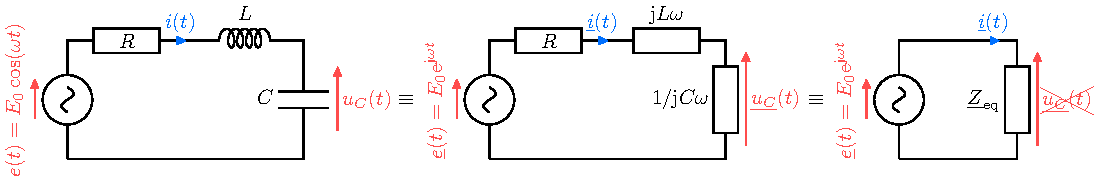
\includegraphics[width=\linewidth, draft=true]{rlc_sinu_zeq}
		}{
			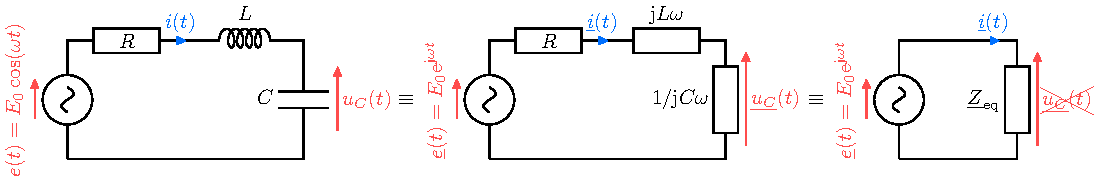
\includegraphics[width=\linewidth]{rlc_sinu_zeq}
		}
		\vspace{-15pt}
		\captionof{figure}{Circuit RLC série et équivalences.}
	\end{minipage}
	\begin{isd}[sidebyside align=top]
		\tcbsubtitle{\fatbox{Amplitudes complexe et réelle}}
		\wsw{
			\begin{DispWithArrows*}[fleqn, mathindent=2pt]
				E_0 = \Zu\ind{eq}\Iu & =
				\left( R + \jlw + \frac{1}{\jcw} \right)\Iu
				\Arrow{On isole}
				\\\Lra
				\Iu                    & =
				\frac{E_0}{R + \jj \left( L\w - \dfrac{1}{C\w} \right)}
				\Arrow{On factorise par $R$}
				\\\Lra
				\Iu                    & =
				\frac{E_0/R}{1 + \jj \left( \dfrac{L}{R}\w  - \dfrac{1}{RC\w}\right)}
			\end{DispWithArrows*}
			De plus,
			\begin{gather*}
				\boxed{\frac{L}{R} = \frac{Q}{\w_0}}
				\qet
				Q\w_0 = \frac{1}{R} \sqrt{\frac{\cancel{L}}{C}} \frac{1}{\sqrt{\cancel{L}C}}
				\Lra
				\boxed{ \frac{1}{RC} = Q\w_0}
				\\\Ra
				\Iu = \frac{E_0/R}{1 + \jj \left( \dfrac{Q\w}{\w_0} - \dfrac{Q\w_0}{\w}
					\right)}
				\Lra
				\boxed{
					\Iu = \frac{E_0/R}{1 + \jj Q \left(
						\dfrac{\w}{\w_0} - \dfrac{\w_0}{\w}
						\right)}}
				\\\Ra
				\boxed{
					I(\w)
					= \abs{\Iu}
					= \frac{E_0/R}{\sqrt{1 + Q^2\left( \dfrac{\w}{\w_0} - \dfrac{\w_0}{\w}
							\right)^2}}
				}
			\end{gather*}
		}
		\vspace{-15pt}
		\tcblower
		\tcbsubtitle{\fatbox{Pulsation de résonance et phase}}
		\wsw{
			On trouve le maximum de cette amplitude quand le dénominateur est minimal,
			c'est-à-dire
			\begin{gather*}
				I(\w_r) = I_{\max}
				\Lra
				1 + Q^2\left( \frac{\w_r}{\w_0} - \frac{\w_0}{\w_r} \right)^2 \text{minimal}\\
				\Lra
				Q^2\left( \frac{\w_r}{\w_0} - \frac{\w_0}{\w_r} \right)^2 = 0
				\Lra
				\boxed{\w_r = \w_0}
			\end{gather*}
			Pour la phase~:
			\begin{gather*}
				\f_i
				= \underbrace{\cancel{\arg*{E_0/R}}}_{=0}
				- \arg*{1 + \jj Q \left(
					\frac{\w}{\w_0} - \frac{\w_0}{\w}
					\right)}
				\\\Lra
				\boxed{\tan\f_i = -Q\left( \frac{\w}{\w_0} - \frac{\w_0}{\w} \right)}
				\qavec
				\boxed{\f_i \in \left] - \frac{\pi}{2}\,; \frac{\pi}{2} \right[}
			\end{gather*}
			puisque $\cos\f_i > 0$ (la partie réelle est positive).
			\begin{align*}
				\tan\f_i \xrightarrow[\w\to0^+]{} +\infty
				\Ra &
				\boxed{\f_i \xrightarrow[\w\to0^+]{} +\frac{\pi}{2}}
				\\
				\tan(\f_i(\w_0)) =0
				\Ra &
				\boxed{\f_i(\w_0) = 0}
				\\
				\tan\f_i \xrightarrow[\w\to+\infty]{} -\infty
				\Ra &
				\boxed{\f_i \xrightarrow[\w\to0^+]{} - \frac{\pi}{2}}
			\end{align*}
		}
		\vspace{-15pt}
	\end{isd}
	\noindent
	\begin{minipage}[]{\linewidth}
		\centering
		\sswitch{
			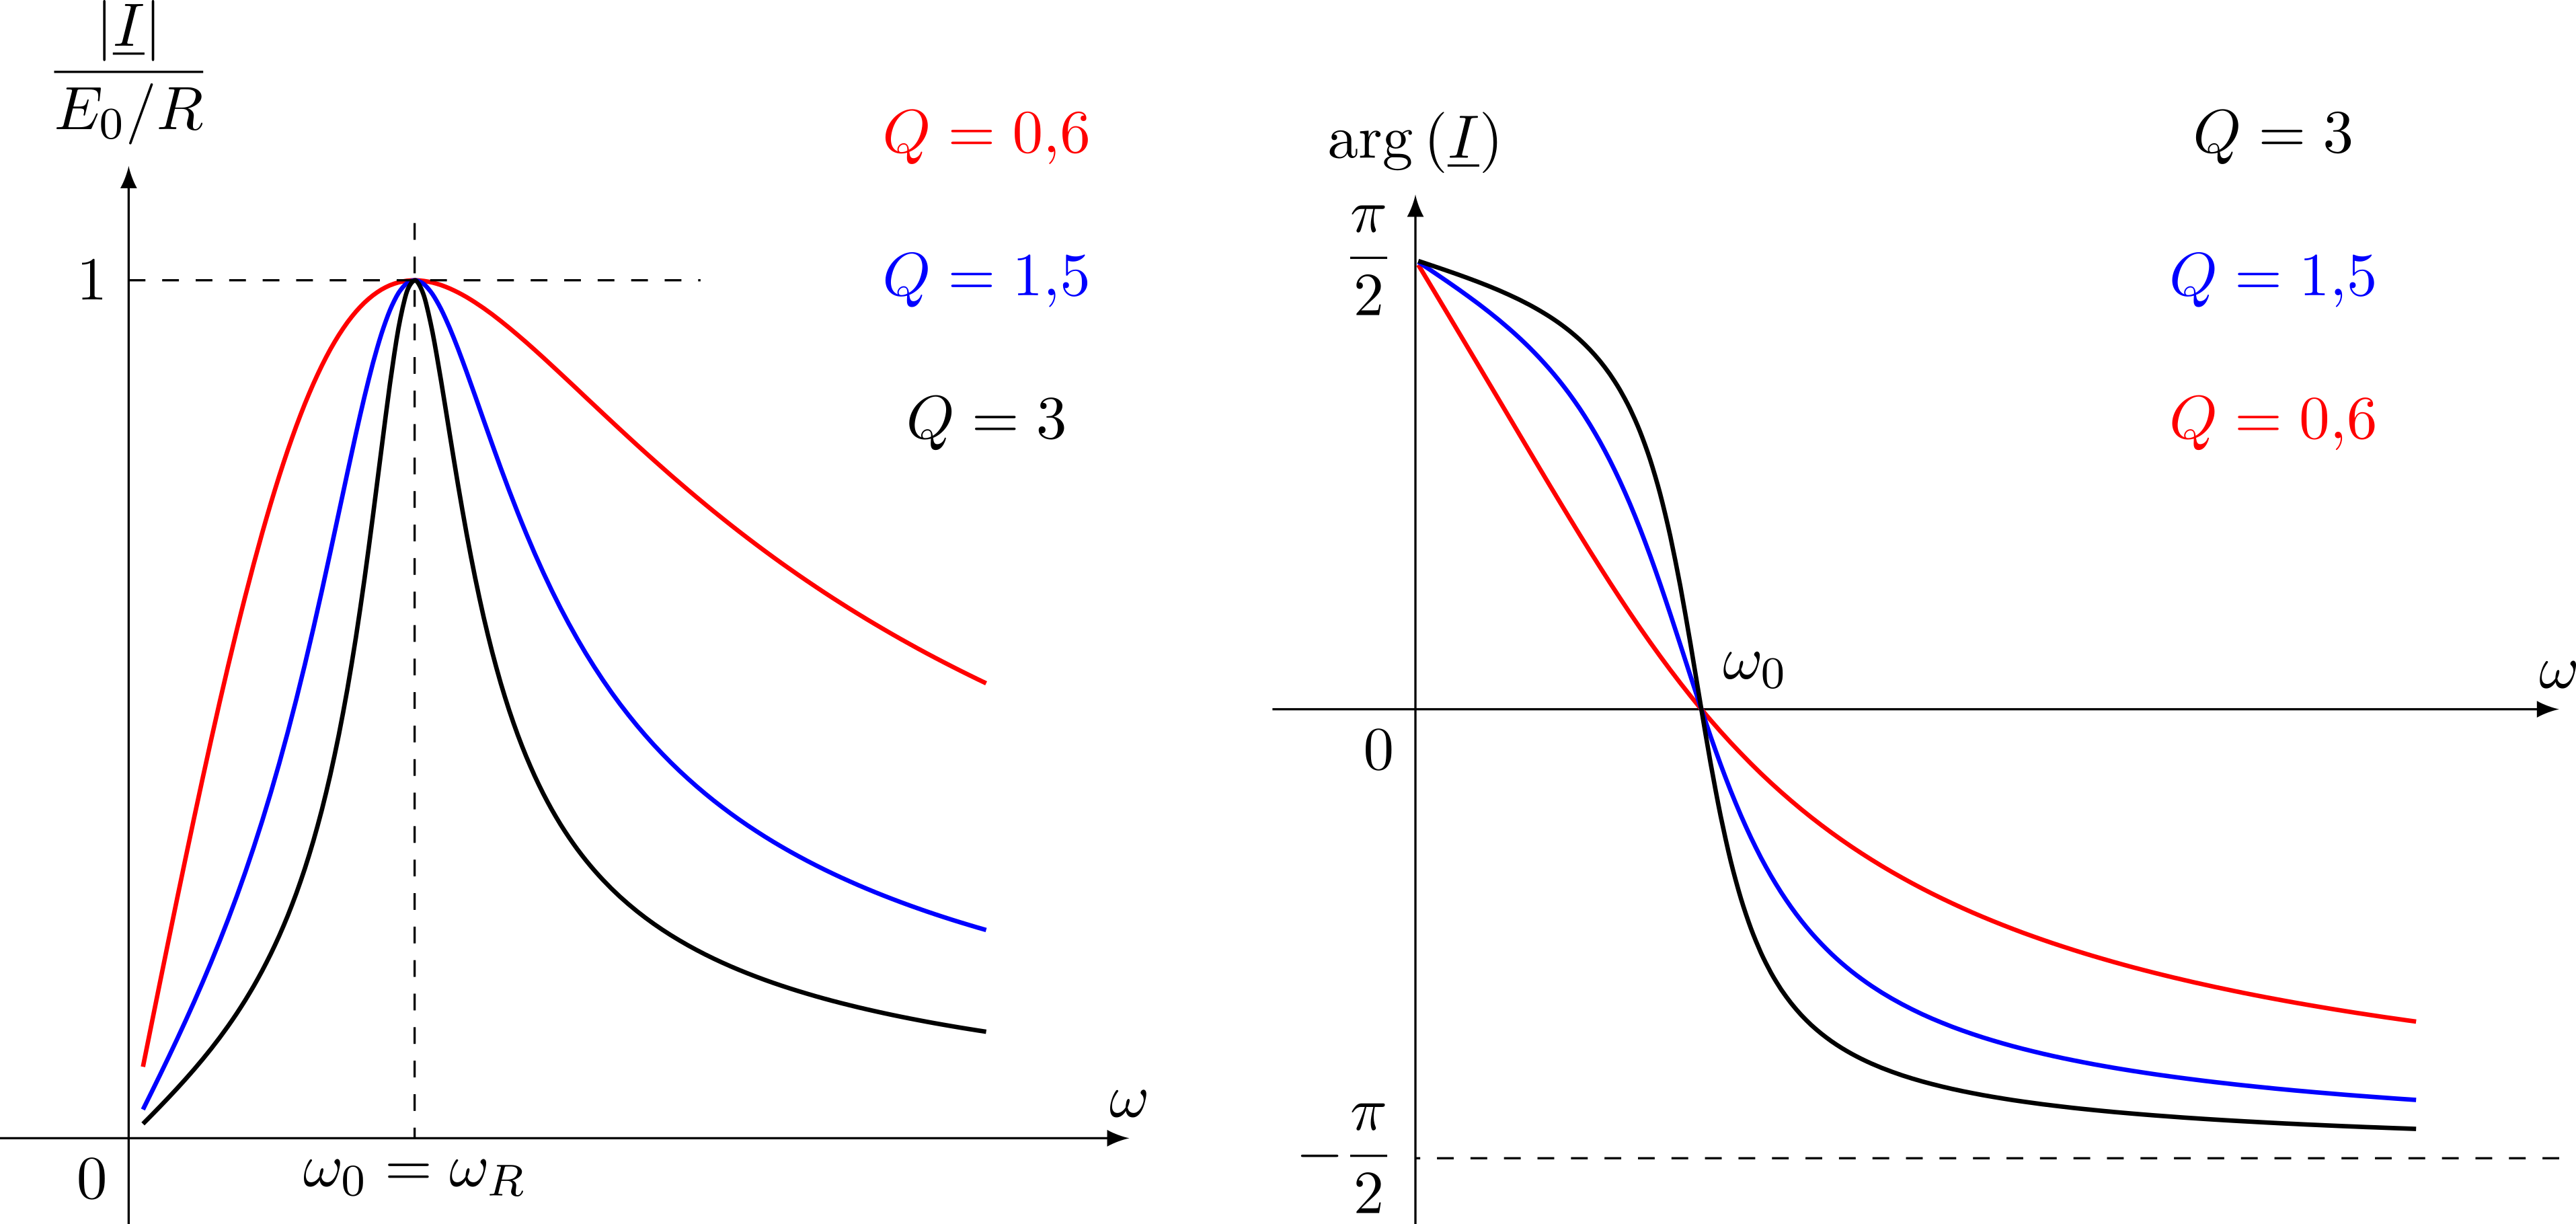
\includegraphics[width=.8\linewidth, draft=true]{rlc_i-ampphase}
		}{
			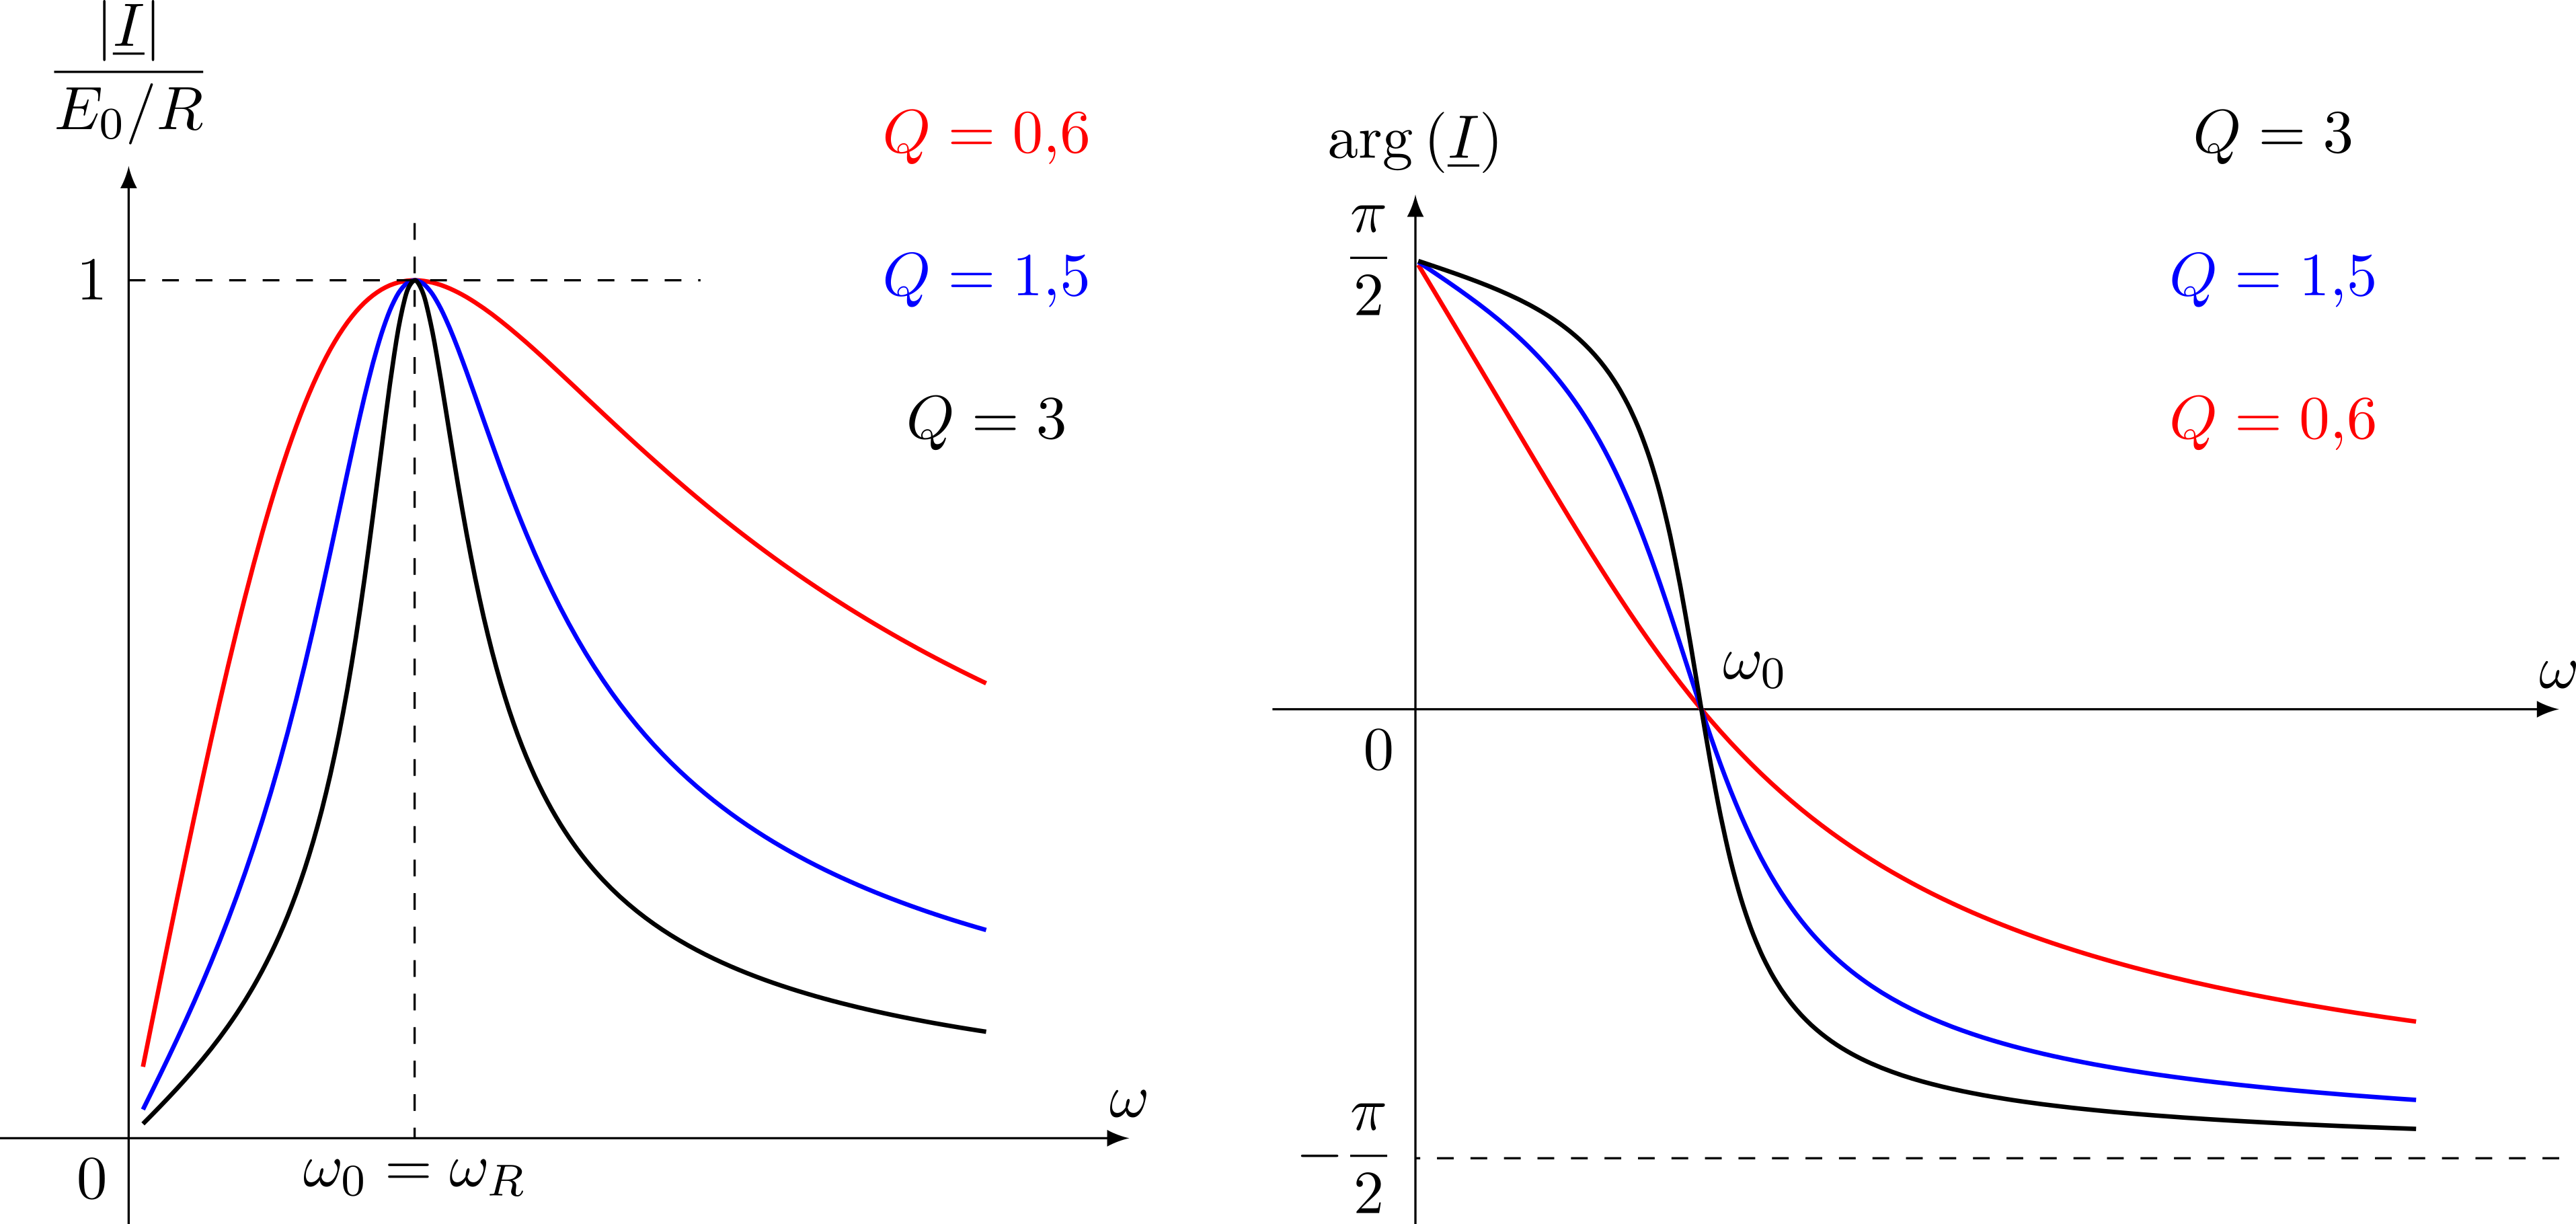
\includegraphics[width=.8\linewidth]{rlc_i-ampphase}
		}
		\captionof{figure}{Amplitude et phase en fonction de $Q$ pour $\Iu$ en RLC
			série.}
	\end{minipage}
	\vspace*{-30pt}
	\ifstudent{
		\begin{tikzpicture}[remember picture, overlay]
			\node[anchor=north west, align=left]
			at ([shift={(1.4cm,0)}]current page.north west)
			{\\[5pt]\Large\bfseries Nom~:\\[10pt]\Large\bfseries Prénom~:};
			\node[anchor=north east, align=right]
			at ([shift={(-1.5cm,-17pt)}]current page.north east)
			{\Large\bfseries Note~:\hspace{1cm}/10};
		\end{tikzpicture}
	}
\end{enumerate}
\end{document}
